% Commented HMDf tala patterns latex code moved to the end
Similar to Carnatic music, we do corpora level analysis of rhythm patterns\index{Rhythm pattern} in Hindustani music and illustrate several musicological inferences and insights, and contrast if there are any differences between music theory and practice. The rhythm patterns described in this section were obtained using spectral flux, in an identical process as described for Carnatic music. % \comment{explain further: what are these differences ?}

The \figrefs{fig:tt:HMDl:teen}{fig:tt:HMDs:rupak}\ show the cycle length rhythm patterns for all \glspl{taal} for both \acrshort{HMDl} and \acrshort{HMDs} datasets, using the spectral flux feature computed identically to the way it was computed for Carnatic music rhythm patterns, as an average over the entire dataset indicated. In each figure, the bottom pane corresponds to the low frequency band ($\protect\obsLow$) and the top pane corresponds to the high frequency band ($\protect\obsHigh$). The abscissa is the \gls{matra} number within the cycle (dotted lines), with 1 indicating the \gls{sam} (marked with a red line). The start of each \gls{vibhaag} is indicated at the top of each pane (\gls{sam} shown as $\times$).

The rhythm patterns in Hindustani are indicative of \gls{tabla} strokes played in the cycle. In the figures, the bottom pane that shows the low frequency band has content from the \gls{bayan} (the left bass drum) of the \gls{tabla} while the top pane has content predominantly from the \gls{dayan} (the right pitched drum) of the \gls{tabla}, but additionally from the lead melody. Hence, for the purpose of this discussion, we use the terms left and right accents to refer to the accents in rhythm patterns from the bottom and top pane, respectively. 

The left and right accents provide interesting insights into the patterns played within a \gls{taal} cycle. We additionally compare rhythm patterns across the \glspl{lay} by plotting the patterns for \acrshort{HMDl} dataset (with \gls{vilambit} \gls{lay} pieces) and \acrshort{HMDs} dataset (\gls{madhyam} and \gls{dhrut} lay pieces) - for each \gls{taal}, the patterns for these two data subsets are plotted in two figures one below the other.

The patterns played in a \gls{taal} cycle have both energy/amplitude accents due to varying strength of the \gls{tabla} stroke and also timbral characteristics, due to the specific stroke played. The rhythm patterns have been generated using the spectral flux feature, which models mostly only energy, and hence can only explain energy accents with these figures. We list down and discuss some salient qualitative observations from the figures for each \gls{taal}, for both \gls{vilambit} \gls{lay} and \gls{madhyam}/\gls{dhrut} \gls{lay}. The patterns are indicative of the surface rhythm present in these audio recordings.

There are several observations from the plotted rhythm patterns that have interesting musicological significance. A professional Hindustani musician has informally validated these observations, but they still have to be formally studied in depth to make valid musicological conclusions. Overall, from \figrefs{fig:tt:HMDl:teen}{fig:tt:HMDs:rupak}, we observe across all \glspl{taal} and \glspl{lay} that accents are stronger on the \glspl{matra}, with accents present even at half and fourth divisions of the matra in many cases. The \gls{sam} most often has the strongest accent. Unlike Carnatic \glspl{tala}, \glspl{theka} in Hindustani music are less flexible, and hence we can infer several concrete conclusions from the rhythm patterns of Hindustani music. 

Across all \glspl{taal} in \gls{vilambit} \gls{lay}, we see additional filler strokes present between \glspl{matra}, showing that percussionists add further metrical subdivisions lower than the \gls{matra}, though not defined in theory. These fillers are also mostly concentrated towards the second half of the \gls{matra}. The 1\tsup{st} \gls{matra} (and often the 2\tsup{nd} \gls{matra}) is quite empty with few accents, while the last few \glspl{matra} of the cycle have dense accents. This is to place a special emphasis on the \gls{sam}, indicating the approaching of \gls{sam} with fillers and dense stroke playing, while there is a short recovery period after the \gls{sam} with fewer strokes. In addition, a dense matra with many fillers is often followed by a sparsely accented \gls{matra} to better contrast the progression through the \gls{taal} cycle, e.g. a dense \gls{matra} 9 after a quieter \gls{matra} 8 in \figref{fig:tt:HMDl:teen}. %and \gls{madhyam} 

Due to the large \gls{matra} period ($\ibi$) in \gls{vilambit} \gls{lay}, each \gls{matra} acts as an anchor for timekeeping, and can be played without any effect from the previous strokes (in fast \gls{tabla} playing in \gls{dhrut}, the previous stroke can possibly affect the sound, intonation, and playing technique of the following strokes). Further, due to a large time interval available to play the \gls{theka}, the \gls{tabla} playing musician focuses on modulation of left bass strokes that can sustain longer. Finally, left and right hand can operate independently, which means modulation of accents through the cycle can be different for left and right accents. The left and right strokes also complement each other. Each of these effects can be observed in the patterns of \gls{vilambit} \gls{lay}. % 

In contrast, across all \glspl{taal} in \gls{madhyam} and \gls{dhrut} \gls{lay}, given the shorter cycles, we see that \glspl{vibhaag} are anchors. The fillers are largely restricted only to half \gls{matra}, with lower accents. \Gls{dhrut} pieces also have a relatively more relaxed timing, and the focus is on right strokes, with the left hand playing the theory defined ``textbook” strokes for timekeeping. In addition, the left and right hands are in sync, which can be seen in the modulation of accents through the cycle being well correlated for both left and right accents - the left and right strokes work together here, in contrast to complementing each other as in \gls{vilambit} \gls{lay}. Furthermore, the patterns differ widely between the \gls{lay} classes, especially for \gls{ektal} and \gls{teental}. 

We now present some \gls{taal} specific observations from the rhythm patterns for each \gls{taal}. Some of these observations corroborate the theory while some of them show the contrast between theory and practice. These inferences mainly address \gls{tabla} stroke playing during the cycles, while the effects of melody has not been considered into account. This is a valid assumption to make since these patterns are averaged over several cycles, averaging out and reducing the effect of melody on these rhythm patterns. 
% Tala pattern: HMDl-teen-all-lo230-superflux-mvavg-normZ, HMDl-teen-all-hi250-superflux-mvavg-normZ
\begin{figure}[t]
\captionsetup[subfigure]{labelformat=empty}
\centering
\subfloat[]{\label{fig:tt:HMDl:teen:hi}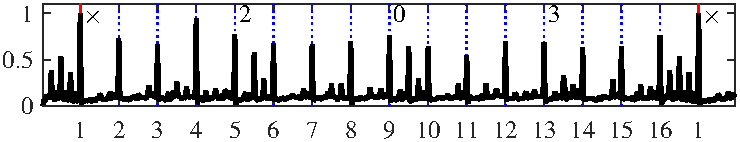
\includegraphics[width=\textwidth]{talaPatts/HMDl-teen-all-hi250-superflux-mvavg-normZ.pdf}} \\ \vspace{-1.35cm}
\subfloat[]{\label{fig:tt:HMDl:teen:lo}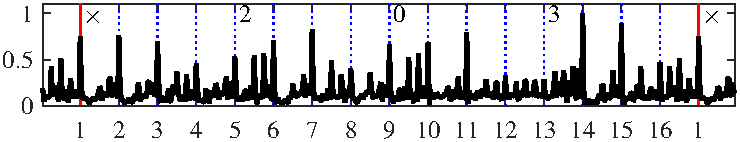
\includegraphics[width=\textwidth]{talaPatts/HMDl-teen-all-lo230-superflux-mvavg-normZ.pdf}}
\caption[Rhythm patterns in \gls{teental} learned from \acrshort{HMDl} dataset]{Cycle length rhythmic patterns learned from \acrshort{HMDl} dataset for \gls{teental}, computed from spectral flux feature and averaged over all the pieces in the dataset. The bottom/top pane corresponds to the low/high frequency bands, respectively. The abscissa is the \gls{matra} number within the cycle (dotted lines), with 1 indicating the \gls{sam} (marked with a red line). The start of each \gls{vibhaag} is indicated at the top of each pane (\gls{sam} shown as $\times$). The plot shows the cycle extended by a \gls{matra} at the beginning and end to illustrate the cyclic nature of the \gls{taal}.}\label{fig:tt:HMDl:teen} % HMDl-teen-all-hi250-superflux-mvavg-normZ,HMDl-teen-all-lo230-superflux-mvavg-normZ
\end{figure}
% , computed from spectral flux feature and averaged over all the pieces in the dataset. The bottom/top pane corresponds to the low/high frequency bands, respectively. The abscissa is the \gls{matra} number within the cycle (dotted lines), with 1 indicating the \gls{sam} (marked with a red line). The start of each \gls{vibhaag} is indicated at the top of each pane (\gls{sam} shown as $\times$).
% 
%
% Tala pattern: HMDs-teen-all-lo230-superflux-mvavg-normZ, HMDs-teen-all-hi250-superflux-mvavg-normZ
\begin{figure}[t]
\captionsetup[subfigure]{labelformat=empty}
\centering
\subfloat[]{\label{fig:tt:HMDs:teen:hi}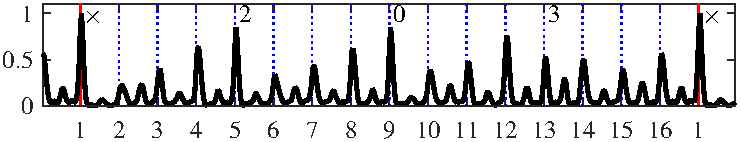
\includegraphics[width=\textwidth]{talaPatts/HMDs-teen-all-hi250-superflux-mvavg-normZ.pdf}} \\ \vspace{-1.35cm}
\subfloat[]{\label{fig:tt:HMDs:teen:lo}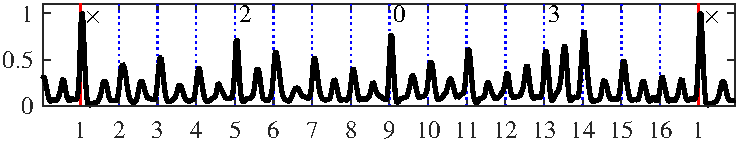
\includegraphics[width=\textwidth]{talaPatts/HMDs-teen-all-lo230-superflux-mvavg-normZ.pdf}}
\caption[Rhythm patterns in \gls{teental} learned from \acrshort{HMDs} dataset]{Cycle length rhythmic patterns learned from \acrshort{HMDs} dataset for \gls{teental}.}\label{fig:tt:HMDs:teen}
\end{figure}
%
%
% From \figrefs{fig:tt:HMDl:teen}{fig:tt:HMDs:teen}
\begin{description}[style=unboxed,leftmargin=0cm]
\item[\textbf{\Gls{vilambit} \gls{teental}}:] From \figref{fig:tt:HMDl:teen}, we see that the 14\tsup{th} matra has the strongest left accent, and the last \gls{matra} (matra 16) has many fillers, both to indicate the arrival of \gls{sam} - a phenomenon known in music theory as \gls{amad} (literal meaning - the approach). A strong left accent on the 9\tsup{th} matra is not defined in theory (the stroke in the \gls{theka} is a right stroke \syl{NA}), but often a \syl{DHA} is played instead. This is a known (to practising musicians) difference between theory and practice and can additionally be observed in the patterns too. As described earlier, the right stroke fillers are fewer in \glspl{matra} 1 and 2, and the left accents support the timekeeping task when the right accents are weaker there. 4\tsup{th} \gls{matra} has a strong right accent perhaps to indicate the end of the 1\tsup{st} \gls{vibhaag}, after a filler-less \glspl{matra} 2 and 3. The beginning of the 2\tsup{nd} and 3\tsup{rd} \glspl{vibhaag}, labeled 2 and 0 have higher number of fillers. The left accents between the 11\tsup{th} and the 14\tsup{th} matra are weak - with the 11\tsup{th} and 14\tsup{th} \gls{matra} accents acting as anchors for the ``quiet" created in between them. It is interesting to note the varying modulation of accent levels through the \glspl{vibhaag} of the cycle. Specifically, we can see that the left and right accent envelopes through the cycle are complementary, indicating that left and right drums are complementary in \gls{vilambit} \gls{lay}. % 5th matra has complementary left and right accents, stronger second filler left accent compared to stronger first filler left accent - why ? (Many a places the bol "Dha - Dha Ge" is played where the second filler 'Ge' is a only-left stroke resulting in relatively higher accent (as the 'Dha' preceding to that also has a right accent))
%
\item[\textbf{\Gls{madhyam} and \gls{dhrut} \gls{lay} \gls{teental}}:] From \figref{fig:tt:HMDs:teen}, we see that the filler strokes in \gls{dhrut} \gls{teental} are restricted to a single filler at half \gls{matra} positions in contrast to three of more fillers in \gls{vilambit}. The accents are more regular due to higher tempi associated. Similar to \gls{vilambit}, the 9\tsup{th} matra has a strong left accent, which again is a well known difference between theory and practice. The 11\tsup{th} and 14\tsup{th} \glspl{matra} have strong left accents to support the build up of accents through \glspl{matra} 12-14 and indicate the arrival of sam (\gls{amad}). It is interesting to note that the right accent at \gls{vibhaag} boundary (\gls{matra} 13) is weaker than that at the previous \gls{matra} 12. This is perhaps due to the stroke on \gls{matra} 13 being skipped and a strong left stroke on \gls{matra} 14 often played to indicate the approaching \gls{sam}. 
%\end{description}
%\begin{description}[style=unboxed,leftmargin=0cm]
\item[\textbf{\Gls{vilambit} \gls{ektal}}:] From \figref{fig:tt:HMDl:ek}, we see that the last matra of the cycle before the \gls{sam} (\gls{matra} 12) has dense accents, with the final filler strokes having stronger left accents than the \gls{sam}. This is another example of \gls{amad}, where the approach of a \gls{sam} is distinctly indicated. The \glspl{matra} 4 and 10 (both with the \gls{theka} \gls{bol} \syl{TI} \syl{RA} \syl{KI} \syl{TA}, see \tabref{fig:theka:hindustani}) have equal accents in theory. However, \gls{matra} 10 has stronger accents than 4 in practice since it is closer to the \gls{sam}. \syl{TI} \syl{RA} \syl{KI} \syl{TA} is often played with more than four strokes towards the end of the matra 4 and 10. Since \syl{TI} \syl{RA} \syl{KI} \syl{TA} is dense, the \gls{matra} following them (\glspl{matra} 5 and 11) have less fillers. In addition, only \glspl{matra} 4 and 10 have fillers distributed throughout the \gls{matra}, while the rest have fillers only towards the end. \Glspl{vibhaag} 2 and 3 (spanning \glspl{matra} 3-6) and \glspl{vibhaag} 5 and 6 (spanning \gls{matra} 9-$\times$) are identical in theory, but we can see several deviations in performance, with \glspl{vibhaag} 5 and 6 having stronger left accents since they are closer to \gls{sam}. Further, the strokes \syl{DHIN} at \gls{matra} 1 and \gls{matra} 2 are identical in theory, but in practice the \syl{DHIN} at \gls{matra} 2 is played softer to differentiate it from the \syl{DHIN} at the \gls{sam}. The modulation of right accent levels through the cycle is interesting, with stronger accents occurring when the \gls{matra} is less dense with lesser number of accents. This has a functional role in timekeeping - aided by stronger accents and denser \glspl{matra}, which complement each other. 
\end{description}
%
% Tala pattern: HMDl-ek-all-lo230-superflux-mvavg-normZ, HMDl-ek-all-hi250-superflux-mvavg-normZ
\begin{figure}[t]
\captionsetup[subfigure]{labelformat=empty}
\centering
\subfloat[]{\label{fig:tt:HMDl:ek:hi}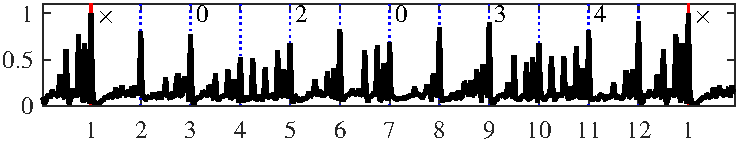
\includegraphics[width=\textwidth]{talaPatts/HMDl-ek-all-hi250-superflux-mvavg-normZ.pdf}} \\ \vspace{-1.35cm}
\subfloat[]{\label{fig:tt:HMDl:ek:lo}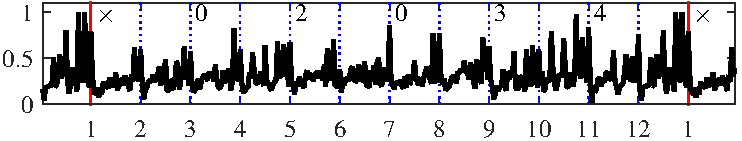
\includegraphics[width=\textwidth]{talaPatts/HMDl-ek-all-lo230-superflux-mvavg-normZ.pdf}}
\caption[Rhythm patterns in \gls{ektal} learned from \acrshort{HMDl} dataset]{Cycle length rhythmic patterns learned from \acrshort{HMDl} dataset for \gls{ektal}.}\label{fig:tt:HMDl:ek}
\end{figure}
%
% Tala pattern: HMDs-ek-all-lo230-superflux-mvavg-normZ, HMDs-ek-all-hi250-superflux-mvavg-normZ
\begin{figure}[t]
\captionsetup[subfigure]{labelformat=empty}
\centering
\subfloat[]{\label{fig:tt:HMDs:ek:hi}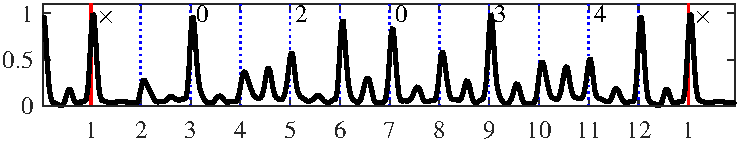
\includegraphics[width=\textwidth]{talaPatts/HMDs-ek-all-hi250-superflux-mvavg-normZ.pdf}} \\ \vspace{-1.35cm}
\subfloat[]{\label{fig:tt:HMDs:ek:lo}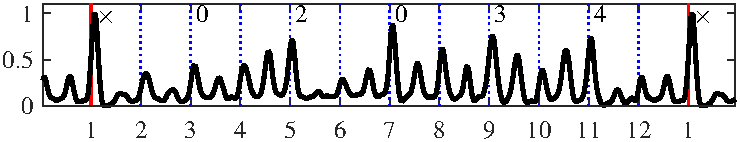
\includegraphics[width=\textwidth]{talaPatts/HMDs-ek-all-lo230-superflux-mvavg-normZ.pdf}}
\caption[Rhythm patterns in \gls{ektal} learned from \acrshort{HMDs} dataset]{Cycle length rhythmic patterns learned from \acrshort{HMDs} dataset for \gls{ektal}.}\label{fig:tt:HMDs:ek}
\end{figure}
%
%
% Tala pattern: HMDl-jhap-all-lo230-superflux-mvavg-normZ, HMDl-jhap-all-hi250-superflux-mvavg-normZ
\begin{figure}[t]
\captionsetup[subfigure]{labelformat=empty}
\centering
\subfloat[]{\label{fig:tt:HMDl:jhap:hi}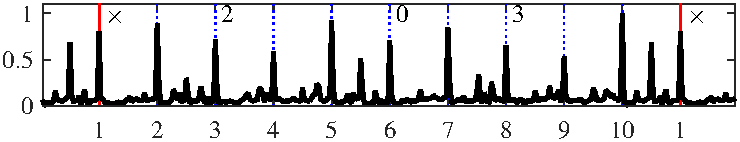
\includegraphics[width=\textwidth]{talaPatts/HMDl-jhap-all-hi250-superflux-mvavg-normZ.pdf}} \\ \vspace{-1.35cm}
\subfloat[]{\label{fig:tt:HMDl:jhap:lo}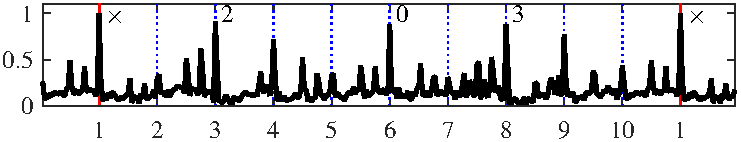
\includegraphics[width=\textwidth]{talaPatts/HMDl-jhap-all-lo230-superflux-mvavg-normZ.pdf}}
\caption[Rhythm patterns in \gls{jhaptal} learned from \acrshort{HMDl} dataset]{Cycle length rhythmic patterns learned from \acrshort{HMDl} dataset for \gls{jhaptal}.}\label{fig:tt:HMDl:jhap}
\end{figure}
%
% Tala pattern: HMDs-jhap-all-lo230-superflux-mvavg-normZ, HMDs-jhap-all-hi250-superflux-mvavg-normZ
\begin{figure}[t]
\captionsetup[subfigure]{labelformat=empty}
\centering
\subfloat[]{\label{fig:tt:HMDs:jhap:hi}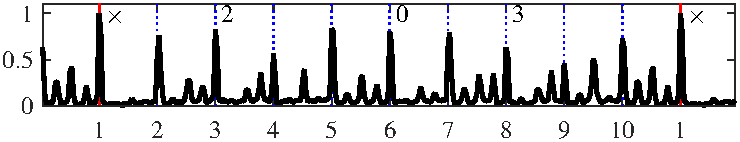
\includegraphics[width=\textwidth]{talaPatts/HMDs-jhap-all-hi250-superflux-mvavg-normZ.pdf}} \\ \vspace{-1.35cm}
\subfloat[]{\label{fig:tt:HMDs:jhap:lo}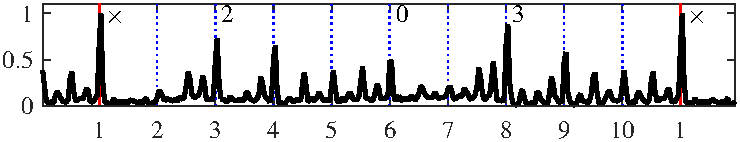
\includegraphics[width=\textwidth]{talaPatts/HMDs-jhap-all-lo230-superflux-mvavg-normZ.pdf}}
\caption[Rhythm patterns in \gls{jhaptal} learned from \acrshort{HMDs} dataset]{Cycle length rhythmic patterns learned from \acrshort{HMDs} dataset for \gls{jhaptal}.}\label{fig:tt:HMDs:jhap}
\centering
\end{figure}
%
\begin{description}[style=unboxed,leftmargin=0cm]
\item[\textbf{\Gls{madhyam} and \gls{dhrut} \gls{lay} \gls{ektal}}:] Though defined with six \glspl{vibhaag} in theory, \gls{dhrut} \gls{ektal} is described better as having four \glspl{vibhaag} of 3 \glspl{matra} each, as shown in \figref{fig:taal:drutektal}, with the \glspl{vibhaag} starting at \glspl{matra} 1, 4, 7, and 10. As can be seen from \figref{fig:tt:HMDs:ek}, the strong right accents due to \syl{NA} stroke at \glspl{matra} 3, 6, 9 and 12 are distinctly seen. This suggests that for \gls{dhrut} \gls{lay}, timekeeping is done more with the sharp right strokes (e.g. `\syl{NA}' here) and accentuation can even be at non-\gls{vibhaag} marker \glspl{matra} such as 6 and 12. Even though the last \gls{vibhaag} starts on matra 10, there is strong right accent on matra 9, an indication of the approaching \gls{sam} (\gls{amad}). The four strokes in \syl{TI} \syl{RA} \syl{KI} \syl{TA} is often not played in \gls{dhrut}, replacing it with just two strokes \syl{TE} \syl{KE} - we see only two accents in \glspl{matra} 4 and 10. In addition, due to the dense stroke playing on \gls{matra} 4 and 10, the left accents in \gls{matra} 6 and 12 are quiet with relatively weaker accents. Similar to \gls{vilambit} \gls{ektal}, though the first and second matra have equal accented \syl{DHIN} stroke in theory, \syl{DHIN} on the second \gls{matra} is played considerably softer with weak accent. As with all \glspl{taal} in \gls{dhrut} \gls{lay}, the accents on left and right through the cycle are correlated. 
\end{description}
%
% Tala pattern: HMDl-rupak-all-lo230-superflux-mvavg-normZ, HMDl-rupak-all-hi250-superflux-mvavg-normZ
\begin{figure}[t]
\captionsetup[subfigure]{labelformat=empty}
\centering
\subfloat[]{\label{fig:tt:HMDl:rupak:hi}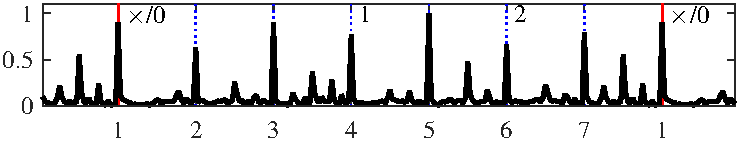
\includegraphics[width=\textwidth]{talaPatts/HMDl-rupak-all-hi250-superflux-mvavg-normZ.pdf}} \\ \vspace{-1.35cm}
\subfloat[]{\label{fig:tt:HMDl:rupak:lo}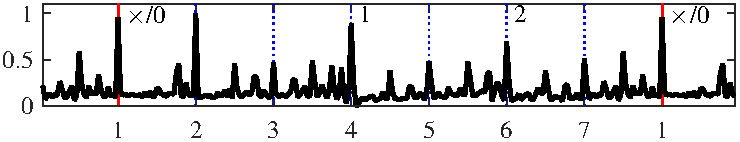
\includegraphics[width=\textwidth]{talaPatts/HMDl-rupak-all-lo230-superflux-mvavg-normZ.pdf}}
\caption[Rhythm patterns in \gls{rupak} learned from \acrshort{HMDl} dataset]{Cycle length rhythmic patterns learned from \acrshort{HMDl} dataset for \gls{rupak}.}\label{fig:tt:HMDl:rupak}
\end{figure}
%
%
% Tala pattern: HMDs-rupak-all-lo230-superflux-mvavg-normZ, HMDs-rupak-all-hi250-superflux-mvavg-normZ
\begin{figure}[t]
\captionsetup[subfigure]{labelformat=empty}
\centering
\subfloat[]{\label{fig:tt:HMDs:rupak:hi}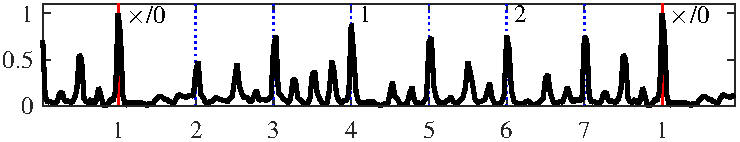
\includegraphics[width=\textwidth]{talaPatts/HMDs-rupak-all-hi250-superflux-mvavg-normZ.pdf}} \\ \vspace{-1.35cm}
\subfloat[]{\label{fig:tt:HMDs:rupak:lo}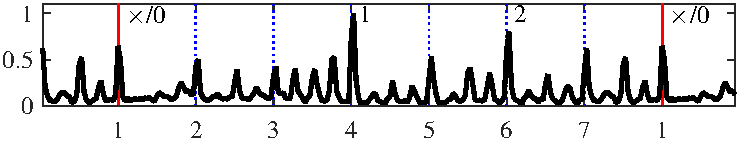
\includegraphics[width=\textwidth]{talaPatts/HMDs-rupak-all-lo230-superflux-mvavg-normZ.pdf}}
\caption[Rhythm patterns in \gls{rupak} learned from \acrshort{HMDs} dataset]{Cycle length rhythmic patterns learned from \acrshort{HMDs} dataset for \gls{rupak}.}\label{fig:tt:HMDs:rupak}
\end{figure}
%
\begin{description}[style=unboxed,leftmargin=0cm]
\item[\textbf{\Gls{vilambit} \gls{jhaptal}}:] From \figref{fig:tt:HMDl:jhap}, we see that all the \syl{NA} strokes (\glspl{matra} 2, 5, 7, 10) have a strong right accent and weak left accents, as described in theory. There are filler strokes to end the \glspl{vibhaag} at \glspl{matra} 2 and 7. This can be explained with the often played variant of the \gls{jhaptal} \gls{theka} (\syl{DHI} \syl{NA-TE-KE} \syl{DHI} \syl{DHI} \syl{NA} | \syl{TI} \syl{NA-TE-KE} \syl{DHI} \syl{DHI} \syl{NA}). There are further strong accented fillers on \glspl{matra} 5 and 10 that act as anchor points to indicate the end of half and full cycle. 
%
\item[\textbf{\Gls{madhyam} and \gls{dhrut} \gls{lay} \gls{jhaptal}}:] \figref{fig:tt:HMDs:jhap} shows that the left accents are as defined in theory with basic \gls{theka} playing. The envelope of accents through the cycle is more regular than in \gls{vilambit} \gls{jhaptal}. In theory, the \gls{vibhaag} 2 (\glspl{matra} 3-5) and \gls{vibhaag} 4 (\glspl{matra} 8-10) are identical, but some deviations can be observed in practice. % (a ``textbook" \gls{bayan} playing)
\end{description}
%
\begin{description}[style=unboxed,leftmargin=0cm]
\item[\textbf{\Gls{vilambit} \gls{rupak}}:] \Gls{rupak} is defined in theory with no left accents on \glspl{matra} 1 and 2, but in practice left strokes are often played (with closed strokes than modulated sustained left strokes). This also implies that \gls{rupak} having a \gls{khali} (0) on the \gls{sam} does not mean it is less accented. \Gls{rupak} is defined to have a 3+2+2 structure, but we see from \figref{fig:tt:HMDl:rupak} that \gls{matra} 2 has a strong left accent, which acts as an anchor, giving the \gls{vilambit} \gls{rupak} a 1+2+2+2 structure, which is close to the tapping of \gls{mishra chapu} \gls{tala} of Carnatic music in practice. This could also be because musicians might play with the same accent on both \syl{TIN} (\glspl{matra} 1 and 2) with a \syl{KAT} stroke to contrast with the \syl{NA} stoke which is less left-accented. The \gls{vibhaag} 2 (\glspl{matra} 4-5) and \gls{vibhaag} 3 (\gls{matra} 6-7) are identical in theory, but in practice the accents differ. \Gls{matra} 5 has the strongest right accent (\syl{NA} stroke), perhaps indicating \gls{amad}. Fillers are more on \gls{matra} 3, to end \gls{vibhaag} 1. In general, we also see that the fillers get more dense towards the end of \glspl{vibhaag}. 
%
\item[\textbf{\Gls{madhyam} and \gls{dhrut} \gls{lay} \gls{rupak}}:] From \figref{fig:tt:HMDs:rupak}, the left strokes and accents closely follow the description in theory. The strongest left accent is on \gls{matra} 4, as defined in theory. The \gls{vibhaag} 2 and 3 are identical with similar accents. Interestingly, the fillers grow through the cycle, becoming more dense towards the end of the cycle. In \gls{dhrut} \gls{rupak}, the accent on the second \gls{matra} is softer than \gls{vilambit} \gls{rupak}, going back to its canonical 3+2+2 structure compared to 1+2+2+2 structure in \gls{vilambit} \gls{rupak}. 
\end{description}
%
% 
%%%%%%%%%%%%%%%%%%%%%%%%%%%%%%%%%%% HMDf tala patterns moved here %%%%%%%%%%%%%%%%%%%%%%%%%
% Tala pattern: HMDf-teen-all-lo230-superflux-mvavg-normZ, HMDf-teen-all-hi250-superflux-mvavg-normZ
% \begin{figure}
% \captionsetup[subfigure]{labelformat=empty}
% \centering
% \subfloat[]{\label{fig:tt:HMDf:teen:hi}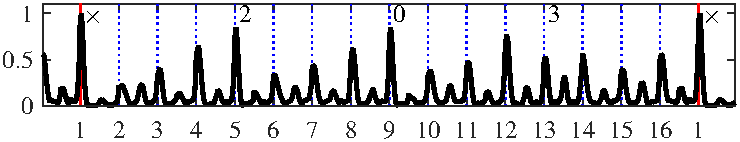
\includegraphics[width=\textwidth]{talaPatts/HMDf-teen-all-hi250-superflux-mvavg-normZ.pdf}} \\ \vspace{-1.35cm}
% \subfloat[]{\label{fig:tt:HMDf:teen:lo}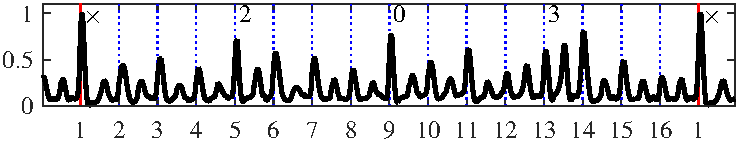
\includegraphics[width=\textwidth]{talaPatts/HMDf-teen-all-lo230-superflux-mvavg-normZ.pdf}}
% \caption[HMDf-teen]{HMDf-teen-all-hi250-superflux-mvavg-normZ,HMDf-teen-all-lo230-superflux-mvavg-normZ}\label{fig:tt:HMDf:teen}
% \end{figure}
%
%
% Tala pattern: HMDf-ek-all-lo230-superflux-mvavg-normZ, HMDf-ek-all-hi250-superflux-mvavg-normZ
% \begin{figure}
% \captionsetup[subfigure]{labelformat=empty}
% \centering
% \subfloat[]{\label{fig:tt:HMDf:ek:hi}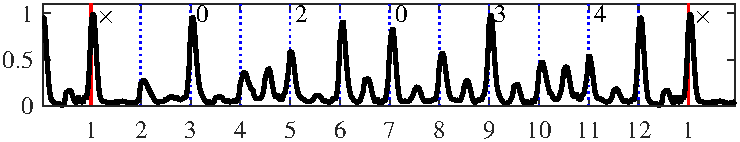
\includegraphics[width=\textwidth]{talaPatts/HMDf-ek-all-hi250-superflux-mvavg-normZ.pdf}} \\ \vspace{-1.35cm}
% \subfloat[]{\label{fig:tt:HMDf:ek:lo}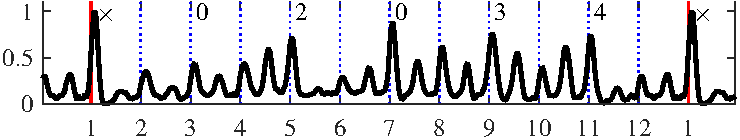
\includegraphics[width=\textwidth]{talaPatts/HMDf-ek-all-lo230-superflux-mvavg-normZ.pdf}}
% \caption[HMDf-ek]{HMDf-ek-all-hi250-superflux-mvavg-normZ,HMDf-ek-all-lo230-superflux-mvavg-normZ}\label{fig:tt:HMDf:ek}
% \end{figure}
%
%
% Tala pattern: HMDf-jhap-all-lo230-superflux-mvavg-normZ, HMDf-jhap-all-hi250-superflux-mvavg-normZ
% \begin{figure}
% \captionsetup[subfigure]{labelformat=empty}
% \centering
% \subfloat[]{\label{fig:tt:HMDf:jhap:hi}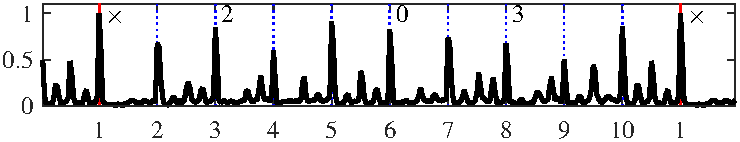
\includegraphics[width=\textwidth]{talaPatts/HMDf-jhap-all-hi250-superflux-mvavg-normZ.pdf}} \\ \vspace{-1.35cm}
% \subfloat[]{\label{fig:tt:HMDf:jhap:lo}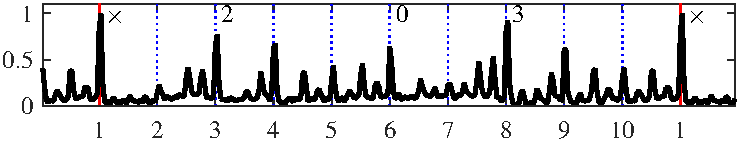
\includegraphics[width=\textwidth]{talaPatts/HMDf-jhap-all-lo230-superflux-mvavg-normZ.pdf}}
% \caption[HMDf-jhap]{HMDf-jhap-all-hi250-superflux-mvavg-normZ,HMDf-jhap-all-lo230-superflux-mvavg-normZ}\label{fig:tt:HMDf:jhap}
% \end{figure}
%
%
% Tala pattern: HMDf-rupak-all-lo230-superflux-mvavg-normZ, HMDf-rupak-all-hi250-superflux-mvavg-normZ
% \begin{figure}
% \captionsetup[subfigure]{labelformat=empty}
% \centering
% \subfloat[]{\label{fig:tt:HMDf:rupak:hi}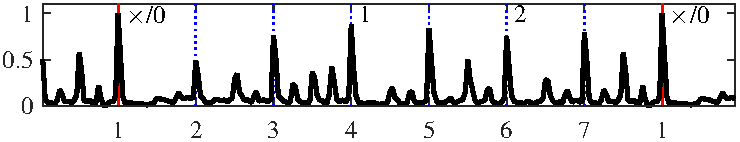
\includegraphics[width=\textwidth]{talaPatts/HMDf-rupak-all-hi250-superflux-mvavg-normZ.pdf}} \\ \vspace{-1.35cm}
% \subfloat[]{\label{fig:tt:HMDf:rupak:lo}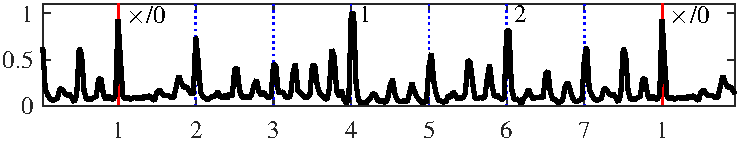
\includegraphics[width=\textwidth]{talaPatts/HMDf-rupak-all-lo230-superflux-mvavg-normZ.pdf}}
% \caption[HMD-rupak]{HMDf-rupak-all-hi250-superflux-mvavg-normZ,HMDf-rupak-all-lo230-superflux-mvavg-normZ}\label{fig:tt:HMDf:rupak}
% \end{figure}
%